%===============================================================
% Chapter 1 — Background and Theoretical Foundations
% Thesis: A Smart Farm IoT Monitoring and Deterministic Agronomic
%         Analytics Platform for Alfalfa Cultivation
% Authors: Abderrahmane Henna · Nacer Eddine Aouissi
% Supervisor: Mohib Eddine KHEBBACHE
% University of El Oued – Echahid Hamma Lakhdar, 2025/2026
%===============================================================

\chapter{Background and Theoretical Foundations}
\label{chap:background}

%---------------------------------------------------------------
\section{Chapter Introduction}
\label{sec:ch1-intro}
%---------------------------------------------------------------

Agricultural monitoring in arid and semi-arid environments requires more than
sensors and wireless links. It demands a coherent understanding of why field data
is collected, what constraints govern collection, how data travels from the field
to storage, and what agronomic context gives measurements meaning. Before
presenting the implemented system, this chapter builds the theoretical and
technical foundation needed to understand the design choices and the problem being
addressed.

The chapter is organized as follows. Section~\ref{sec:saharan-agriculture}
describes the Saharan agricultural context that motivates the project.
Section~\ref{sec:data-collection} discusses the role of structured data collection
in agricultural monitoring. Section~\ref{sec:smart-agriculture-iot} introduces
smart agriculture and the Internet of Things. Sections~\ref{sec:communication}
and~\ref{sec:topologies} examine wireless communication technologies and network
topologies relevant to field IoT deployments. Sections~\ref{sec:low-power}
and~\ref{sec:reliability} address energy management and fault recovery, two
practical constraints that strongly shape embedded system design. Finally,
Sections~\ref{sec:alfalfa-background} and~\ref{sec:why-alfalfa} present the
agronomic context of alfalfa cultivation and explain why it was selected as the
target crop for this work.

%---------------------------------------------------------------
\section{Saharan Agriculture Context}
\label{sec:saharan-agriculture}
%---------------------------------------------------------------

Algeria's agricultural landscape ranges from the fertile Tell Atlas in the north
to vast desert zones in the south, where cultivation depends almost entirely on
underground water resources and careful land management. In Saharan regions such
as the Souf valley, agricultural activity is concentrated in palm-grove oases and
irrigated field plots that have been adapted over generations to extreme
environmental conditions~\cite{hadeid_saharan_agriculture_algerian_oasis}.
% TODO: verify citation metadata for hadeid_saharan_agriculture_algerian_oasis

These conditions present specific challenges that are absent from more temperate
agricultural settings. Summer temperatures regularly exceed 40°C, creating thermal
stress for both crops and embedded electronics. Rainfall is scarce and
unpredictable, making groundwater the primary irrigation source. Groundwater
extraction and distribution must therefore be managed carefully to avoid
overuse~\cite{desert_agriculture_food_security_algeria}.
% TODO: verify citation metadata for desert_agriculture_food_security_algeria

Beyond the climatic constraints, the infrastructure of remote agricultural
plots is often limited. Electrical grid access may be intermittent or absent
entirely, forcing farm equipment and monitoring systems to rely on local power
sources such as batteries or small solar panels. Internet connectivity, where
available, is typically provided by mobile data networks and cannot be assumed to
be stable or continuously available.

Manual monitoring under these conditions is both physically demanding and
practically limited. A farmer who must inspect several widely separated field
plots cannot observe all of them simultaneously, and observations made at
irregular intervals may miss short-duration events such as a sudden temperature
spike or a period of soil drying between irrigation cycles. The consequence is
that agronomic decisions are frequently made on the basis of incomplete or
outdated information.

Digitally supported agriculture in Saharan regions has attracted growing interest
as a way to address this monitoring gap. Some work has explored applying smart
agriculture techniques specifically to desert and oasis contexts in
Algeria~\cite{smart_agriculture_desert_wadi_souf}, recognizing that the technical
requirements differ substantially from those of more conventional farming
environments.
% TODO: verify citation metadata for smart_agriculture_desert_wadi_souf

The proposed monitoring platform was designed with these constraints explicitly in
mind. Its offline-first architecture, battery-oriented firmware design, and
manual upload mechanism respond directly to the realities of Saharan field
deployment rather than assuming the stable connectivity and power supply typical
of controlled agricultural environments.

%---------------------------------------------------------------
\section{Data Collection in Agriculture}
\label{sec:data-collection}
%---------------------------------------------------------------

A common simplification treats agricultural monitoring as synonymous with sensor
data collection. In practice, the information needed to support field decisions
comes from several distinct sources, each with its own temporal semantics and
reliability characteristics.

The most familiar category is automatic sensor measurements: values produced by
instruments that observe a physical variable at a defined point in space and time.
These readings form the primary signal from which soil and weather trends are
derived. However, sensor readings alone do not tell the full story. They must be
accompanied by structured contextual information: when exactly the reading was
taken, which device produced it, whether the device was operating correctly at
the time, and whether any data was lost before the reading reached its destination.

Teh et al.~\cite{teh2020sensor_data_quality} reviewed the quality challenges
inherent to IoT sensor data at scale and identified completeness, consistency,
timeliness, and accuracy as the four core dimensions of data quality. Any
monitoring system that handles sensor readings without addressing these dimensions
risks producing analytics that are misleading or unverifiable.

A second category of agricultural data concerns operational events generated by
the monitoring system itself. Node failures, communication losses, recovery
actions, and upload completions all produce records that describe the state and
behavior of the infrastructure. These records are not measurements of the field;
they are measurements of the system. Keeping them separate from field measurements
is important for diagnostic clarity.

A third category is manually entered agronomic information: records created by
farm operators to document field actions such as irrigation start and end times,
fertilization events, cutting dates, and observations that would otherwise remain
informal. This information enriches the interpretation of sensor trends but
carries a different reliability profile, since its accuracy depends on the
discipline and precision of the person recording it.

Timestamping is the thread that connects these categories. Dandrifosse et
al.~\cite{dandrifosse2024weather_qc_agriculture} demonstrated in the context of
agricultural weather data that automatic quality control requires unambiguous and
consistent observation timestamps. When the time a measurement was taken differs
from the time it was uploaded, processed, or stored, using the wrong timestamp as
the analytical reference can produce charts and statistics that do not correspond
to actual field conditions. A rigorous data collection system must therefore
separate measurement time from transfer time and maintain that distinction
throughout the data pipeline.

%---------------------------------------------------------------
\section{Smart Agriculture and the Internet of Things}
\label{sec:smart-agriculture-iot}
%---------------------------------------------------------------

The Internet of Things refers to the broad set of technologies and practices by
which physical devices are connected through digital communication infrastructure
to collect, transmit, and exchange data with other systems and with human
users~\cite{gubbi2013iot_vision}. Although the concept applies across many
domains, agriculture has emerged as one of the areas where IoT-based approaches
offer substantial practical benefits.

Smart agriculture applies connected sensing, communication, and computing
technologies to the problems of field monitoring, crop management, irrigation
scheduling, and resource optimization. Ayaz et al.~\cite{ayaz2019iot_smart_agriculture_survey}
surveyed IoT-based smart agriculture across a wide range of deployment
environments and noted that soil condition monitoring, weather observation, and
remote field access are the most frequently addressed use cases. Farooq et
al.~\cite{farooq2019iot_smart_agriculture_review} similarly reviewed the role of
IoT in implementing smart farming practices and emphasized the growing importance
of low-cost embedded systems in making field instrumentation accessible.

A typical IoT agricultural monitoring system can be understood in terms of three
functional layers. The sensing layer consists of embedded nodes equipped with
sensors that observe environmental and soil variables. The communication and
storage layer handles the movement of measurements from field nodes to a backend
system and their preservation for later retrieval. The visualization and
interpretation layer makes stored data accessible to farm operators and analysts
through dashboards and analytics tools.

It is important to distinguish between monitoring systems and control systems.
A monitoring system collects and displays information, supporting human decisions
about irrigation, fertilization, and crop management. A control system goes
further and takes autonomous actions, such as activating a pump when a soil
moisture threshold is reached. The distinction is not only technical; it also
concerns the level of validation and trust that an agronomic claim requires.
A monitoring platform that shows that soil moisture declined after a hot day is
providing information. A system that automatically triggers irrigation based on
that same reading is making an agronomic decision on behalf of the operator.
These two roles carry different responsibilities, and the distinction between
them should be clear in any technical description of a smart agriculture system.

%---------------------------------------------------------------
\section{IoT Communication Technologies}
\label{sec:communication}
%---------------------------------------------------------------

The communication protocol chosen for an IoT field deployment determines the
range over which devices can exchange data, the power they consume while doing so,
the infrastructure they require, and their robustness to outdoor interference.
No single protocol is optimal for all contexts, and the choice must be guided by
the specific requirements of the deployment environment.

\textbf{Wi-Fi} operates in the 2.4\,GHz and 5\,GHz bands and offers high data
throughput at the cost of limited range and relatively high power consumption.
Typical indoor ranges of 30 to 100 metres are rarely sufficient for distributed
field nodes spread across several hundred metres of open agricultural land. Wi-Fi
also requires the deployment and maintenance of access points, which may not be
practical in remote locations.

\textbf{Bluetooth} and \textbf{Bluetooth Low Energy (BLE)} are designed for
short-range device communication, typically within 10 metres. While useful for
local diagnostics and configuration, they are not suited to field monitoring over
distances of more than a few tens of metres.

\textbf{Zigbee} supports mesh networking and operates at ranges of roughly 100 to
300 metres per hop. Its low power characteristics make it appropriate for dense
sensor networks, but its range per hop is still limited for agricultural fields
where nodes may be hundreds of metres from the nearest relay.

\textbf{Cellular (GSM/4G)} networks provide wide-area coverage through existing
infrastructure, eliminating the need for dedicated field gateways. The tradeoffs
are higher power consumption, ongoing subscription costs, and dependency on
network operator coverage, which may be inconsistent in remote agricultural areas.

\textbf{LoRa (Long Range)} is a spread-spectrum modulation technique developed by
Semtech that operates in sub-GHz ISM bands~\cite{semtech2020sx127x_datasheet}.
It achieves ranges of several kilometres in open terrain while maintaining very
low power consumption, making it particularly well suited to battery-powered field
nodes that transmit relatively small data packets at infrequent intervals.
LoRaWAN, defined by the LoRa Alliance specification~\cite{loraalliance2020lorawan_104},
adds a network architecture layer on top of LoRa, specifying gateway behaviour,
device classes, and cloud server communication. However, it is also possible to
use LoRa in a custom point-to-point or star topology without LoRaWAN
infrastructure, which is the approach taken in many agricultural research
prototypes.

Figure~\ref{fig:lora-module-ch1} shows the LoRa transceiver module used in this
project's monitoring nodes. The module's sub-GHz operating frequency provides
better propagation through vegetation and around obstacles compared to higher-
frequency technologies, a relevant advantage in agricultural environments with
irregular terrain and vegetation.

\begin{figure}[H]
  \centering
  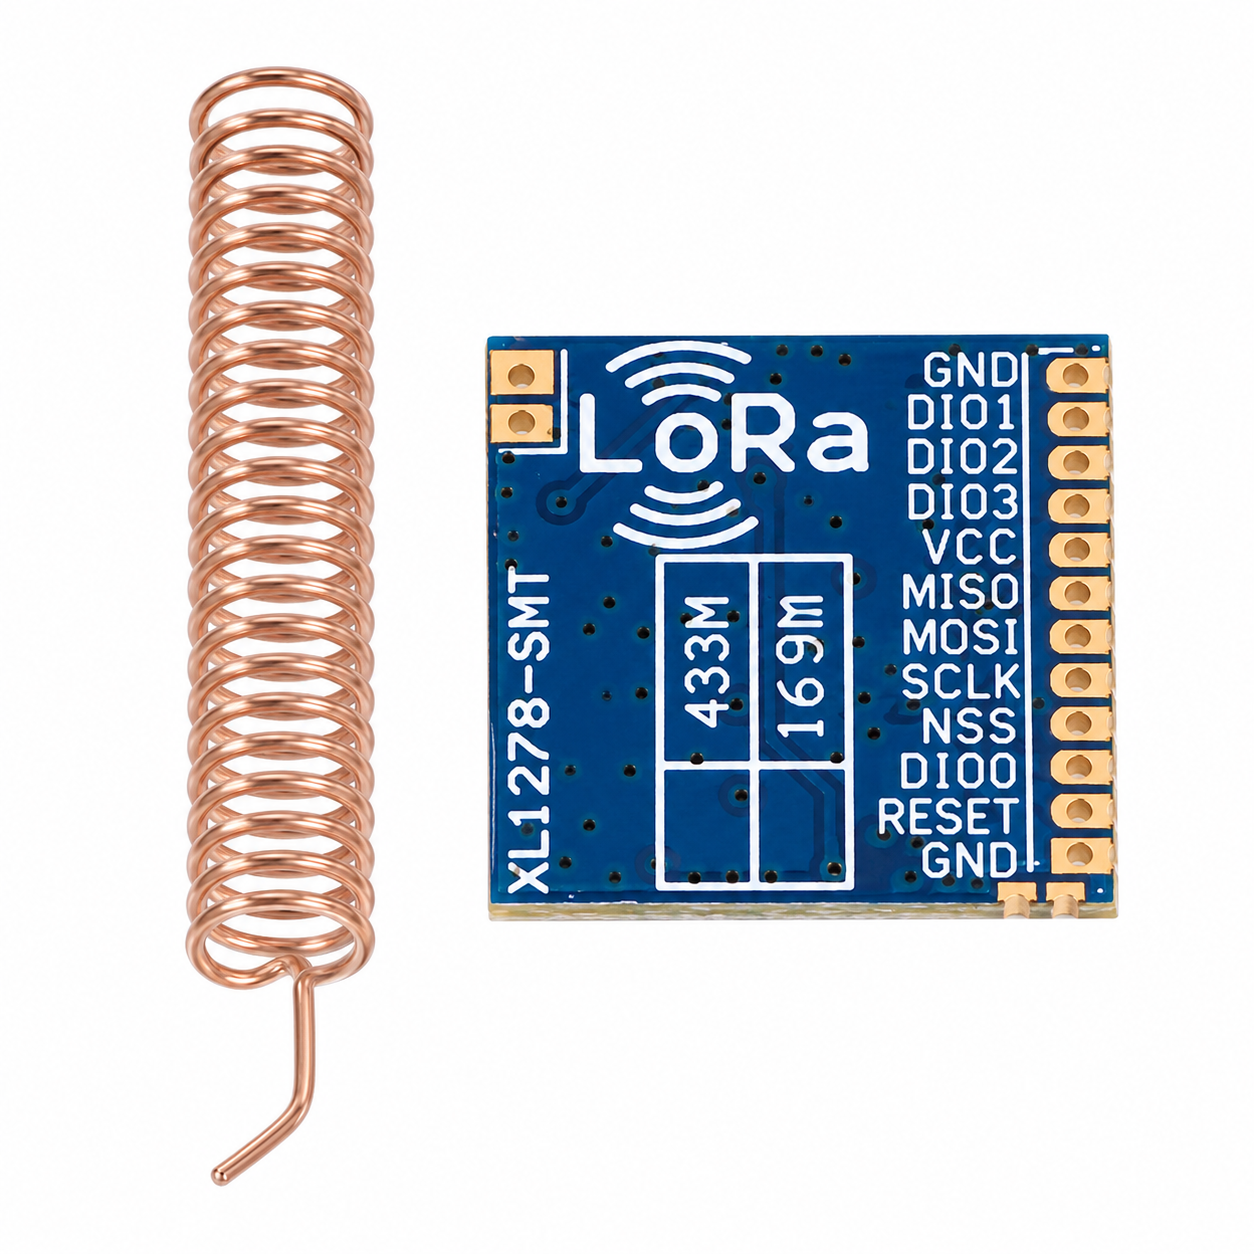
\includegraphics[width=0.45\textwidth]{figures/LoRa}
  \caption{LoRa transceiver module used for long-range wireless communication
           between distributed field nodes and the monitoring gateway.}
  \label{fig:lora-module-ch1}
\end{figure}

Table~\ref{tab:iot-communication-comparison} summarizes the main wireless
communication technologies considered for IoT agricultural field deployments,
comparing them on the criteria most relevant to outdoor, battery-powered, and
infrastructure-limited environments.

\begin{table}[H]
  \centering
  \caption{Comparison of wireless communication technologies for field IoT deployments.}
  \label{tab:iot-communication-comparison}
  \renewcommand{\arraystretch}{1.3}
  \begin{tabular}{|p{2.2cm}|p{2.2cm}|p{2.0cm}|p{2.4cm}|p{2.0cm}|p{2.2cm}|}
    \hline
    \textbf{Technology} & \textbf{Typical range} & \textbf{Power draw} &
    \textbf{Infrastructure} & \textbf{Cost} & \textbf{Field suitability} \\
    \hline
    Wi-Fi & 30–100\,m & Medium–High & Access points required & Low–Medium & Limited \\
    \hline
    Bluetooth/BLE & Up to 10\,m & Low & None & Low & Very limited \\
    \hline
    Zigbee & 100–300\,m per hop & Low & Coordinator node & Low & Moderate \\
    \hline
    GSM/4G & National coverage & High & Cellular network & High & High (where coverage exists) \\
    \hline
    LoRa & 1–15\,km & Very low & Gateway & Low & Very high \\
    \hline
  \end{tabular}
\end{table}

%---------------------------------------------------------------
\section{IoT Network Topologies}
\label{sec:topologies}
%---------------------------------------------------------------

Beyond the physical communication protocol, the arrangement of devices within a
network determines how data flows, where coordination occurs, and how the system
responds to individual node failures.

In a \textbf{point-to-point} topology, two devices communicate directly with each
other. This is the simplest arrangement and is adequate when a single sensor node
reports to a single receiver, but it does not scale to systems with multiple
sensing nodes.

A \textbf{star topology} places a central node, usually called a gateway or
coordinator, at the hub of the network. All sensing nodes communicate directly
with the gateway rather than with each other. The gateway aggregates incoming
measurements, manages acknowledgements, and handles the connection to any upstream
service. This topology is simple to implement, places minimal computational
demands on the sensing nodes, and provides a natural single point for data
collection and forwarding.

A \textbf{mesh topology} allows nodes to relay packets on behalf of each other,
enabling communication between nodes that are not within direct radio range of the
gateway. Mesh networks are more resilient to individual node failures but require
more complex routing protocols and firmware, which increases development effort
and power consumption on each node.

For distributed field monitoring with a small number of sensing nodes spread
across an agricultural site, the star topology is generally the most practical
choice. The gateway can be placed at a location with connectivity access, such as
a point where WiFi or mobile data is reachable for periodic uploads, while the
sensing nodes in the field require only enough radio range to reach it. This
matches the deployment scenario common in IoT agriculture
research~\cite{villa2020iot_arable_farming}.
% TODO: verify citation metadata for villa2020iot_arable_farming

The monitoring system described in this dissertation adopts a gateway-based star
topology using LoRa for field communication. The central gateway node coordinates
data reception from remote sensing nodes, manages local storage, and handles the
upload of collected measurements to the backend service. This organization aligns
with the topological principles described in this section and addresses the
practical constraints of field deployment outlined in
Section~\ref{sec:saharan-agriculture}.

%---------------------------------------------------------------
\section{Low-Power Operation in Field IoT Systems}
\label{sec:low-power}
%---------------------------------------------------------------

Battery-powered embedded nodes represent the practical reality of most distributed
agricultural deployments. Mains power is rarely accessible at precise sensor
placement locations within a field, and running power cables across dozens or
hundreds of metres introduces installation cost, maintenance burden, and the risk
of physical damage. The consequence is that the firmware design of a field node
must treat power consumption as a primary constraint rather than an afterthought.

The fundamental strategy in low-power embedded systems is to minimize the time
a device spends in high-power operating states. Modern microcontrollers support
deep sleep modes in which most internal peripherals are powered down and only
a timer or interrupt source remains active. During deep sleep, current draw can
fall several orders of magnitude below the active-mode consumption. A node that
wakes briefly to take a measurement, transmits a short packet, and returns to
sleep for several minutes or hours can operate for months on a modest battery.

\textbf{Duty cycling} is the general name for this wake-measure-sleep pattern.
Its effectiveness depends on keeping both the active period and the data volume
small. Sensor measurements are typically brief; the slower cost is often radio
communication, especially when retries or acknowledgement windows extend the
transmission period.

Peripheral power control is another dimension of low-power design. Sensors that
draw continuous current even when not being read can dominate the energy budget
of a sleeping device. Connecting such sensors through a relay or transistor switch
allows the microcontroller to power them only during measurement, eliminating
standby drain. Figure~\ref{fig:relay-power-control-ch1} shows the relay module
used in this project to control sensor power during low-power field operation.

\begin{figure}[H]
  \centering
  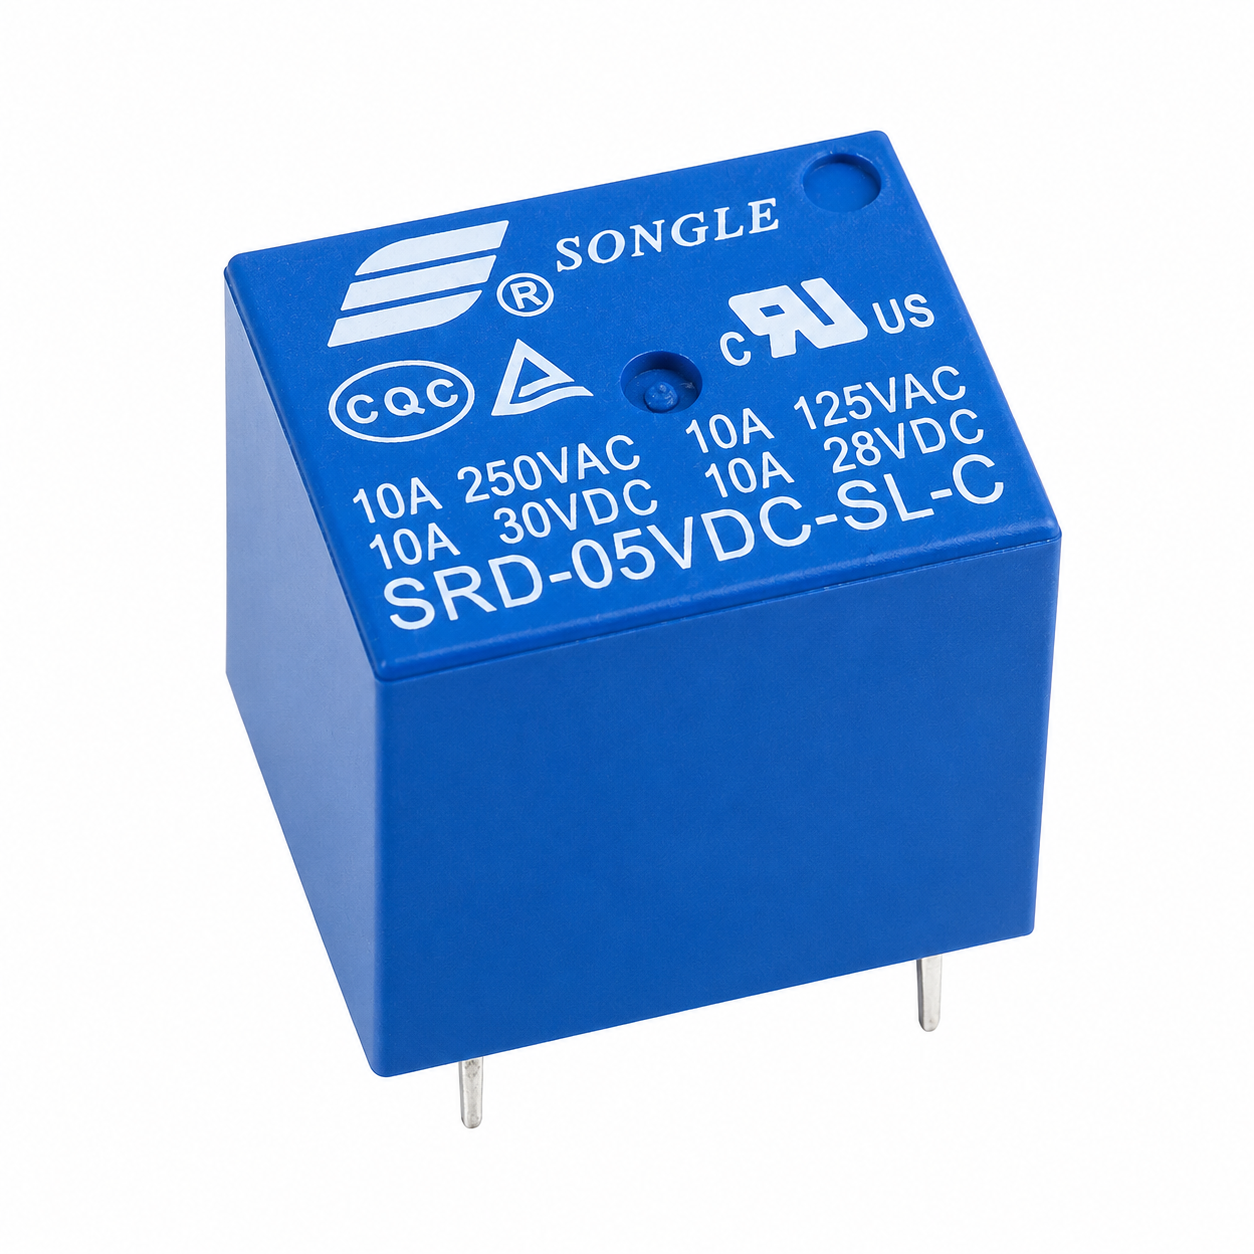
\includegraphics[width=0.35\textwidth]{figures/Relay}
  \caption{Relay module used to control sensor power, enabling measurement on
           demand while eliminating standby current consumption during sleep intervals.}
  \label{fig:relay-power-control-ch1}
\end{figure}

Environmental sensors present a specific case. The BME280 combined temperature,
humidity, and pressure sensor supports a \textit{forced mode} of operation in
which the sensor takes a single measurement triggered by the host microcontroller
and then returns to sleep automatically~\cite{bosch2024bme280_datasheet}. This
eliminates the need for the host to poll the sensor repeatedly or to manage its
active/sleep transitions manually, and it reduces both power consumption and the
risk of register-level programming errors. Figure~\ref{fig:bme280-sensor-ch1}
illustrates the BME280 module as used in the weather sensing node.

\begin{figure}[H]
  \centering
  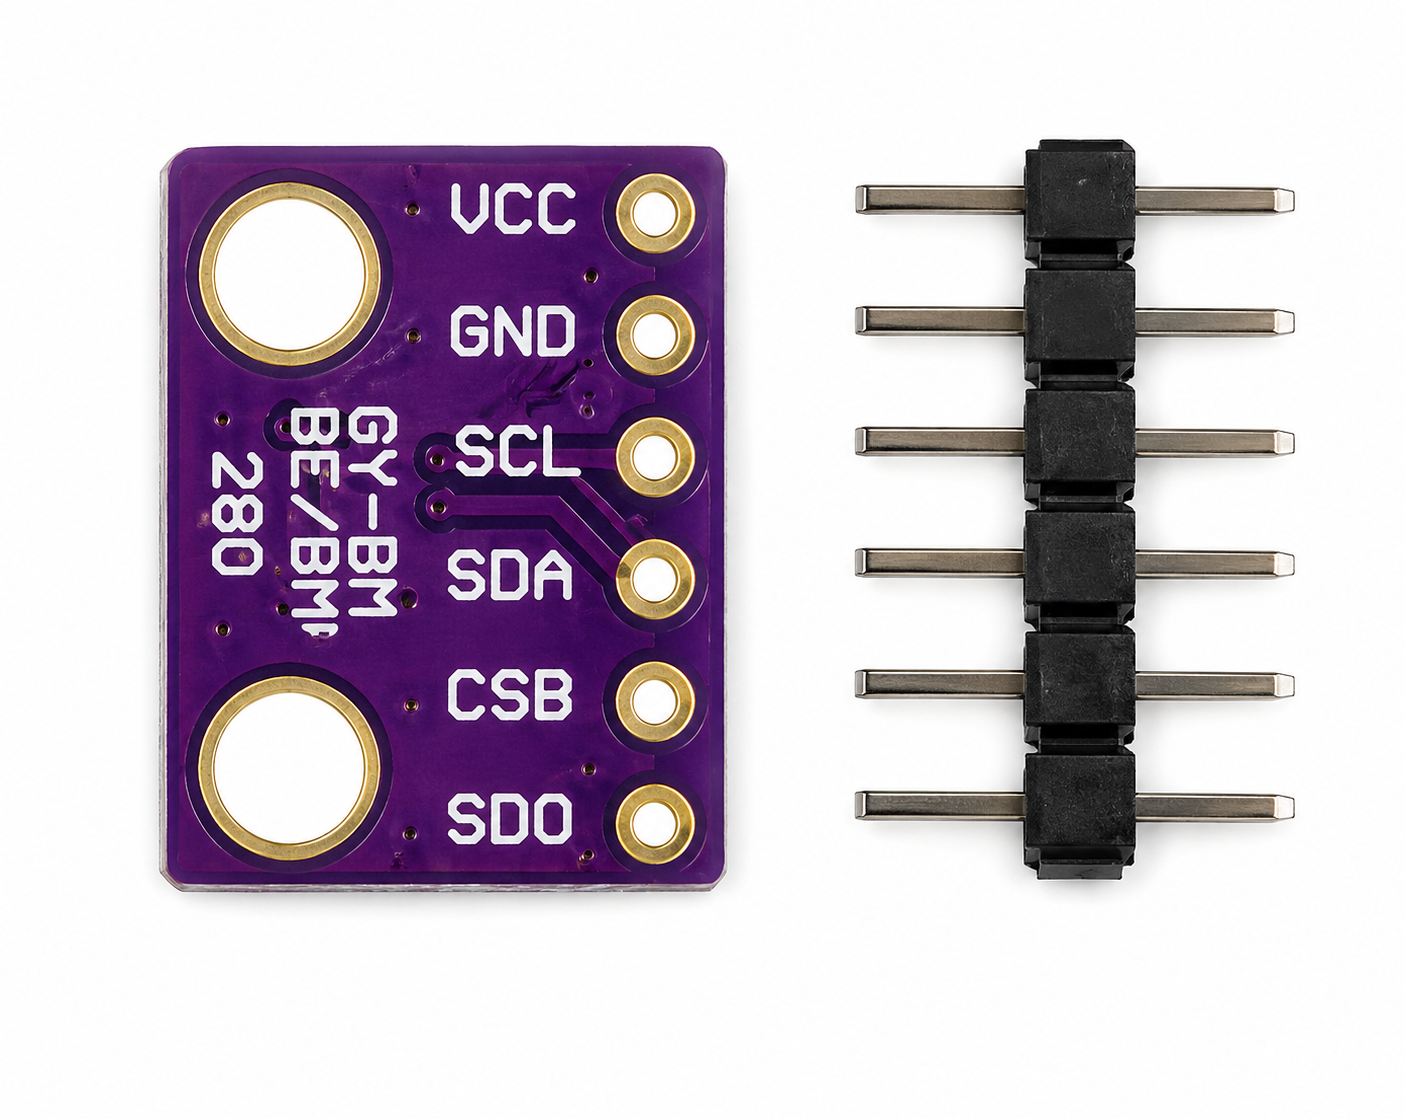
\includegraphics[width=0.40\textwidth]{figures/Bme280}
  \caption{BME280 environmental sensor module providing air temperature, relative
           humidity, and atmospheric pressure measurements in forced measurement mode.}
  \label{fig:bme280-sensor-ch1}
\end{figure}

The combination of deep sleep, duty cycling, relay-controlled sensor power, and
forced measurement mode allows a battery-powered field node to maintain a
meaningful measurement cycle over extended periods without requiring manual
intervention for battery replacement. The exact autonomy achievable depends on
battery capacity, cycle interval, and LoRa transmission parameters, and it
should be characterized experimentally for any specific deployment.

%---------------------------------------------------------------
\section{Reliability and Fault Recovery in IoT Systems}
\label{sec:reliability}
%---------------------------------------------------------------

The outdoor field environment is not a controlled laboratory. Radio signals are
subject to path loss, fading caused by vegetation or terrain, and interference
from other devices operating in the same frequency band. A packet that was
reliably received in bench testing may be lost when the gateway and node are
separated by a row of trees or when the antenna is positioned close to a metallic
surface. This variability is inherent to wireless communication and cannot be
eliminated entirely through hardware selection alone.

The practical consequence is that any field IoT system must be designed around
the assumption that some fraction of transmitted packets will not be received.
The question is how the system detects and responds to this situation.

An \textbf{acknowledgement} mechanism provides the most direct feedback. After
receiving a valid packet, the gateway transmits a short acknowledgement back to
the sender. If the sender does not receive the acknowledgement within a defined
window, it knows that the original packet may not have been received and can
attempt retransmission. This pattern reduces ambiguity and gives the sensing node
concrete information about whether its data reached the gateway.

Retransmission alone does not address a more subtle problem that can arise in
timed systems: \textbf{synchronization loss}. If a node operates on a fixed duty
cycle and misses several consecutive communication windows, the time offset
between the node's expected transmission window and the gateway's expected
reception window can grow. A node that wakes and transmits outside the gateway's
listening period will consistently fail to be received, even if the radio link is
technically functional. Recovery from this state requires a defined procedure
rather than simple retransmission.

Diagnostic event logging provides another layer of reliability management. When
a node misses its expected window, when the gateway fails to receive a packet it
expected, or when a recovery procedure is triggered, recording these events
creates an observable history of system behaviour. This history is valuable both
for real-time diagnostics and for post-hoc analysis of deployment conditions.
A reliability indicator derived from the ratio of received to expected packets is
one way to translate this event history into a metric that appears in dashboard
visualizations and analytics outputs.

%---------------------------------------------------------------
\section{Alfalfa Crop Background}
\label{sec:alfalfa-background}
%---------------------------------------------------------------

Alfalfa (\textit{Medicago sativa} L.) is a perennial leguminous forage crop grown
across a wide range of temperate, semi-arid, and arid environments. Its primary
agricultural role is as a high-quality animal feed: its leaf and stem biomass
provides a nutritionally dense fodder for cattle, sheep, and other livestock, and
its nitrogen-fixing root systems can contribute to long-term soil
fertility~\cite{fao_alflafa_crop_water}.

\subsection{Growth Cycle and Harvest Management}
\label{subsec:alfalfa-growth}

A distinguishing feature of alfalfa compared to annual crops is its perennial
regrowth habit. After an initial establishment period, the crop can be harvested
repeatedly throughout the growing season. Mueller and Teuber
\cite{mueller2007alfalfa_growth_development} describe typical cut cycles ranging
from four to twelve per year depending on climate, irrigation, and variety,
with each cycle proceeding through vegetative recovery, stem elongation, bud
initiation, and first-flower stages before harvest. The timing of each cut affects
both yield and forage quality: harvesting too early reduces biomass, while
delaying beyond the early flower stage lowers digestibility.

This repeated harvest cycle makes continuous monitoring practically beneficial.
Changes in soil moisture and temperature between cuts influence regrowth speed and
the timing of the next harvest decision. An operator who can observe the trend of
soil moisture following irrigation has better information for adjusting the next
irrigation event and for deciding when conditions are suitable for the next cut.

\subsection{Water and Irrigation Requirements}
\label{subsec:alfalfa-water}

Alfalfa is one of the more water-demanding forage crops, with seasonal
evapotranspiration requirements that vary by climate and
variety~\cite{irmak2007irrigation_alfalfa}. In arid and semi-arid environments,
where rainfall is insufficient to meet this demand, supplemental irrigation is
necessary throughout the growing season. Orloff et
al.~\cite{orloff2015drought_strategies_alfalfa} discuss the consequences of water
deficit at different growth stages and the options available to managers when
water supply is constrained, noting that strategic stress, which allows limited
moisture reduction between cuts, is more tolerable than severe deficit during
early regrowth.

For the monitoring system, these irrigation dynamics translate into a practical
need: soil moisture observations must be available before and after irrigation
events to support timing decisions and to document the effect of each irrigation
on the soil profile. Without this data, irrigation management relies on experience
and fixed schedules rather than observed soil conditions.

\subsection{Temperature Sensitivity and Heat Stress}
\label{subsec:alfalfa-heat}

Alfalfa growth is sensitive to thermal conditions. Wassie et
al.~\cite{wassie2019heat_stress_alfalfa} investigated the effects of elevated
temperatures on alfalfa physiology and observed reductions in photosynthetic rate,
leaf area, and shoot biomass under heat stress conditions. In Saharan regions
where summer temperatures regularly exceed 40°C, heat stress is a realistic
seasonal constraint rather than an exceptional event.

Air temperature monitoring therefore provides agronomically relevant context
beyond simple weather records. Observations of high air temperature during a
sensitive growth stage, cross-referenced with soil moisture and agronomic event
records, can help explain unexpected yield reductions or crop recovery patterns.

\subsection{Soil Conditions and Electrical Conductivity}
\label{subsec:alfalfa-soil}

Alfalfa establishes best in well-drained, slightly alkaline soils. It is
moderately tolerant of salinity but shows yield reductions as soil electrical
conductivity increases beyond threshold
levels~\cite{nrcs1999soil_electrical_conductivity}. In irrigated Saharan soils,
where repeated application of groundwater with variable mineral content can
gradually increase soil salinity, monitoring EC trends over time may reveal
deteriorating conditions before they become visible in plant symptoms.

Benabdelouahab et al.~\cite{benabdelouahab2019sensor_calibration_5te} examined the
laboratory calibration and field validation of a multi-parameter soil sensor
measuring moisture, temperature, and EC, and noted that raw in-situ EC values
depend on water content, temperature, and soil texture. This dependency means
that raw EC readings cannot be directly converted to saturated-paste ECe or to
official salinity classifications without appropriate calibration procedures
and reference soil samples. In the context of this project, soil EC is therefore
treated as a relative trend indicator rather than a diagnostic measurement.

\subsection{Summary of Monitoring Requirements}
\label{subsec:alfalfa-monitoring-summary}

Table~\ref{tab:alfalfa-monitoring-needs} summarizes the key agronomic variables
relevant to alfalfa cultivation and their monitoring significance in the context
of a field IoT platform.

\begin{table}[H]
  \centering
  \caption{Key monitoring variables for alfalfa cultivation and their agronomic
           significance in field IoT deployments.}
  \label{tab:alfalfa-monitoring-needs}
  \renewcommand{\arraystretch}{1.3}
  \begin{tabular}{|p{3.2cm}|p{5.0cm}|p{5.8cm}|}
    \hline
    \textbf{Variable} & \textbf{Agronomic relevance} & \textbf{Monitoring role} \\
    \hline
    Soil moisture & Irrigation scheduling; drought stress assessment;
                    cut-cycle timing & Track trends before and after irrigation;
                    compare pivot zones; support operator decisions \\
    \hline
    Soil temperature & Root zone activity; germination conditions;
                       freeze risk at depth & Contextual complement to air
                       temperature; interpretation of soil moisture trends \\
    \hline
    Soil electrical conductivity & Soil salinity trend; potential mineral
                                   accumulation from irrigation water &
                                   Relative trend indicator only; not a
                                   calibrated salinity diagnosis \\
    \hline
    Air temperature & Heat stress risk; growing-degree accumulation;
                      frost risk monitoring & Shared environmental context
                      for both pivot zones \\
    \hline
    Relative humidity & Vapour pressure deficit estimation; atmospheric
                        demand context & Weather context supporting
                        interpretation of soil moisture trends \\
    \hline
    Atmospheric pressure & General weather context; pressure trend
                           monitoring & Supporting environmental variable \\
    \hline
  \end{tabular}
\end{table}

%---------------------------------------------------------------
\section{Why Alfalfa Was Selected}
\label{sec:why-alfalfa}
%---------------------------------------------------------------

The selection of alfalfa as the target crop for this monitoring platform was not
arbitrary. It reflects a combination of regional economic relevance, practical
monitoring need, and a gap in the existing literature.

\subsection{Regional Importance and Demand}
\label{subsec:alfalfa-regional-importance}

Livestock production in Algeria and across the Maghreb region depends heavily on
cultivated fodder crops. Alfalfa is among the most productive and nutritionally
valuable options available, and its perennial nature means that a single
establishment investment supports multiple years of harvest. In the El Oued
region, alfalfa is cultivated in irrigated plots alongside other Saharan
agricultural products, and its contribution to local livestock feed supply gives
it direct economic significance.

The combination of high water demand, repeated cutting cycles, and sensitivity to
temperature and soil conditions makes alfalfa a crop where the benefits of
continuous automated monitoring are especially clear. A farmer managing several
pivot irrigation zones cannot practically visit each one after every cutting event
to assess soil recovery conditions. Remotely accessible, structured field data
fills this gap.

\subsection{The Crop-Specific Monitoring Gap}
\label{subsec:alfalfa-gap}

Reviewing the published literature on IoT-based agricultural monitoring reveals
that the majority of existing systems target general crops, greenhouse environments,
or irrigation automation without specifying the crop or focusing on its particular
monitoring requirements. Soil moisture sensing, LoRa communication, and web-based
dashboards appear frequently in the reviewed works, but alfalfa as a named target
crop is conspicuously absent from the systems encountered in this
review~\cite{ahmed2022lora_agriculture_chile,pereira2023esp32_drip_irrigation,saban2023smart_agricultural_lora_cloud}.

Within Algerian and Saharan agricultural research, some work has addressed desert
agriculture digitalization and smart agriculture applications at a general
level~\cite{iot_enhancements_algerian_desert_agriculture}.
% TODO: verify citation metadata for iot_enhancements_algerian_desert_agriculture
However, the combination of alfalfa crop focus, Saharan field conditions,
offline-first data collection, and deterministic analytics has not been
explicitly addressed in the works identified during the literature review
process. This gap is not stated as a universal absolute; it reflects the scope
of the works reviewed. It is nonetheless a meaningful observation that justifies
the specific framing of this project.

\subsection{Multiple Cutting Cycles as a Monitoring Driver}
\label{subsec:alfalfa-cycles}

The repeated-harvest nature of alfalfa distinguishes it from annual crops in a
way that is particularly relevant to monitoring system design. Each cutting event
resets the soil moisture dynamic: root zone activity temporarily declines, water
uptake slows, and the soil dries differently than during active vegetative growth.
Post-cut irrigation and its effect on soil moisture recovery are therefore
observable events that a time-series monitoring system can capture and document.

For a monitoring platform that separates manual agronomic event records from
automatic sensor measurements, this cycle provides a natural opportunity for
contextual alignment. Recorded irrigation events can be compared with observed
soil moisture trends, and the time between cutting and regrowth can be tracked
against environmental conditions. These are the kinds of relationships that
structured agricultural data makes possible — not as automatic agronomic
decisions, but as information that supports better-informed human decisions.

%---------------------------------------------------------------
\section{Chapter Summary}
\label{sec:ch1-summary}
%---------------------------------------------------------------

This chapter established the theoretical and contextual foundations on which the
proposed monitoring platform is built. The starting point was the Saharan
agricultural environment: harsh temperatures, scarce rainfall, unstable power
supply, and remote field locations that make continuous manual monitoring both
impractical and insufficient.

The discussion of agricultural data collection highlighted that sensor readings
alone are not enough. Traceability, timestamp integrity, and domain separation
between measurements, events, transfer records, and agronomic context are
necessary conditions for data that can be reliably analysed and interpreted.
The smart agriculture and IoT background showed that effective monitoring systems
are organized in layers, with clear responsibilities at each stage of the data
lifecycle, and that the distinction between monitoring and autonomous control has
practical consequences for what a system can and cannot claim.

The communication technology comparison demonstrated why LoRa is well-suited to
distributed field monitoring over distances typical of agricultural sites, given
its combination of range, low power consumption, and freedom from cellular
infrastructure. The network topology discussion reinforced the suitability of
a gateway-based star arrangement for coordinating a small number of sensing nodes
with a central collection point.

Low-power operation and fault recovery were presented as two constraints that
every field IoT design must address explicitly. Deep sleep, duty cycling,
peripheral power control, acknowledgement-based communication, and diagnostic
event logging are not optional refinements; they are design requirements for
systems intended to operate reliably in environments where power is limited and
radio communication is imperfect.

Finally, the alfalfa agronomic background connected the technical infrastructure
to its intended purpose. Soil moisture, soil temperature, soil electrical
conductivity, air temperature, humidity, and atmospheric pressure are the
variables that matter for the crop. The repeated harvest cycle creates natural
opportunities for structured observation, and the absence of dedicated alfalfa
monitoring studies in local Saharan contexts provides a specific motivation for
this work.

The following chapter examines how related works have approached agricultural IoT
monitoring, identifies what they contribute and where their limitations lie, and
uses this comparative analysis to position the proposed system within the broader
field of smart agriculture research.
